\documentclass{article}
\usepackage{tikz}
\usetikzlibrary{decorations.markings}
\usepackage{amsmath}
\usepackage{amsfonts}

\DeclareMathOperator{\HH}{H}
\DeclareMathOperator{\Hom}{Hom}
\DeclareMathOperator{\Gal}{Gal}
\DeclareMathOperator{\GL}{GL}
\DeclareMathOperator{\PGL}{PGL}
\DeclareMathOperator{\PGSp}{PGSp}


\newcommand{\HT}[1]{\widehat{\HH}^{#1}}
\newcommand{\T}{\mathbf{T}}
\newcommand{\Th}{\hat{\T}}
\newcommand{\CC}{\mathbb{C}}

\title{Rectifiers}
\author{Moshe Adrian and David Roe}
\date{\today}

\begin{document}
\maketitle

\section{Questions}

\begin{enumerate}
\item Prove that the character $\chi$ of the coinvariants that Gross gives you, agrees with the cohomology class $c_L$ of the group of type $L$, when restricted to $\HT{-1}$.

We wrote down the following diagram.

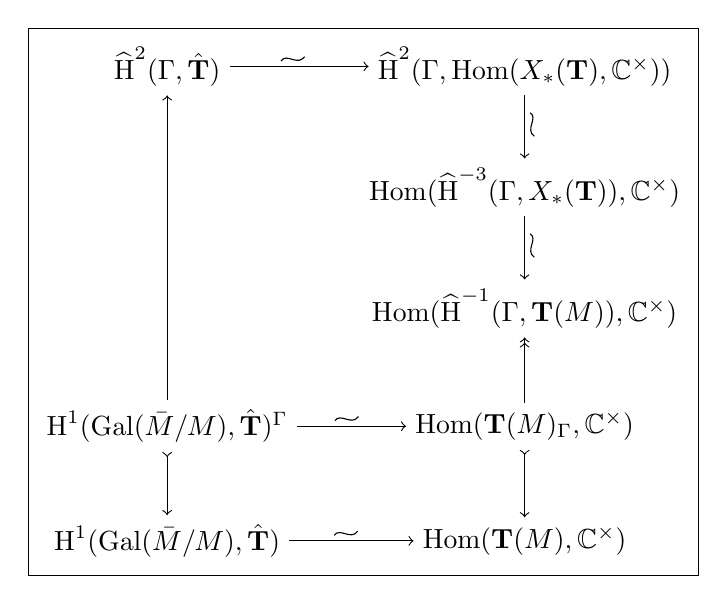
\begin{tikzpicture}[iso/.style={postaction={decorate,decoration={markings, mark=at position 0.45 with {\draw [-] (-4pt,2pt) .. controls (-2pt,5pt) and (2pt, 0pt) .. (4.5pt, 3.5pt);}}}}]
\matrix [draw,nodes=draw,row sep=8mm,column sep=8mm,every node/.style={line width=0pt}]
{
  \node (n00) {$\HT{2}(\Gamma, \Th)$}; & \node (n01) {$\HT{2}(\Gamma, \Hom(X_*(\T), \CC^\times))$}; \\
  & \node (n11) {$\Hom(\HT{-3}(\Gamma, X_*(\T)), \CC^\times)$}; \\
  & \node (n21) {$\Hom(\HT{-1}(\Gamma, \T(M)), \CC^\times)$}; \\
  \node (n30) {$\HH^1(\Gal(\bar{M}/M), \Th)^{\Gamma}$}; & \node (n31) {$\Hom(\T(M)_{\Gamma}, \CC^\times)$}; \\
  \node (n40) {$\HH^1(\Gal(\bar{M}/M), \Th)$}; & \node (n41) {$\Hom(\T(M), \CC^\times$)}; \\
};
\draw [->, iso] (n00) to (n01);
\draw [->, iso] (n01) to (n11);
\draw [->, iso] (n11) to (n21);
\draw [->>] (n31) to (n21);
\draw [>->] (n31) to (n41);
\draw [->, iso] (n30) to (n31);
\draw [->, iso] (n40) to (n41);
\draw [>->] (n30) to (n40);
\draw [->] (n30) to (n00);
\end{tikzpicture}

The arrow $\HH^1(\Gal(\bar{M}/M), \Th)^{\Gamma} \rightarrow \HH^2(\Gamma, \Th)$ fits into the inflation-restriction sequence
\begin{multline*}
0 \rightarrow \HH^1(\Gamma, \Th) \rightarrow \HH^1(\Gal(\bar{M}/K), \Th) \rightarrow \\
 \HH^1(\Gal(\bar{M}/M), \Th)^\Gamma \rightarrow \HH^2(\Gamma, \Th) \rightarrow \HH^2(\Gal(\bar{M}/K), \Th).
 \end{multline*}

So if we want the diagram to commute then we would hope that $\HH^2(\Gal(\bar{M}/K), \Th)$ would vanish....

\item We have defined a base point Langlands parameter that we want to give the correct rectifier.  What difference does it make to send Frobenius to the Tits group element than to any other lift of the Weyl group element defining the group of type $L$?  Answer : We figured out that it doesn't matter if $G$ is semisimple.  But if $G = \GL_2$, then it does matter, we can't just pick any lift.  We have to pick Tits group element (up to a sign?)

\item Let $w$ be an elliptic element of a Weyl group.  Let $\sigma_w$ be the Tits group lift.  Under what conditions is the order of $w$ equal to the order of $\sigma_w$?  This would say that the group of type $L$ splits.  But more generally, under what conditions is there a lift of $w$ that has the same order of $w$?  This would also say that the group of type $L$ splits, so we don't just want to look at the Tits group lift.  We just want to ask when can we lift $w$ to an element in the normalizer that has the same order as $w$. (right?)

\item Check that our conjectural rectifier agrees with the rectifiers for $\PGL_2(F)$, $\PGSp_4(F)$, $\GL_n(F)$, $\PGL_n(F)$ and for all semisimple groups in the DeBacker/Reeder setup.  Partial Answer: We already checked that if $G$ is semisimple, we get the correct rectifier in the DeBacker/Reeder setup. We also checked that we get the same rectifier for $\GL_n(F)$ where $n$ is prime, if the Langlands parameter is tame.

\item Can we use the central character to help us in the case that $\HT{0}$ is nontrivial?  That is, Gross's groups of type $L$ gives us a character on the image of the norm map, which is a subgroup of $T(F)$.  So we don't get a full character of $T(F)$ from Gross's groups of type $L$.  But can we combine what we do get, with a conjectural central character, to get a full character of $T(F)$?

\item In a case outside of DeBacker/Reeder, do we get various expected properties of $L$-packets?

\item What about $\GL_2(F)$, in the ramified situation?  Can we get the rectifier naturally here?  That would be great if we could.

\item Sending Frobenius to the Tits group element is natural because sending to other choices of lifts of the Weyl group element give you the wrong rectifier.

\item Our rectifier agrees with $\GL_n(F)$ in the tame case and $n$ prime.  Does it agree with $\GL_n(F)$ in the tame case where $n$ is arbitrary?  That would be really great.  Start with $\GL_4(F)$, then move on to $\GL_6(F)$ maybe.

\item I have a write-up of various results about tori, unramified in particular.  In the notes $\HT{-1}$ and $\HT{0}$ are calculated in general, for compact unramified tori.  I know you have calculated $\HT{0}$ in your thesis, but I didn't see $\HT{-1}$.  I have a very nice write-up of both of this stuff, and I think we should include it in our paper.

\item Suppose that $w \in W$ is an element of the Weyl group of order $n$, and suppose that $\sigma(w)$ is the Tits group element lifting $w$.  Then
$$\sigma(w)^n = \exp\left(\pi i \sum_{j=0}^{n-1} w^j \cdot \rho^\vee\right),$$
where $\rho^{\vee}$ is half the sum of positive roots.

\end{enumerate}

\section{Outline}

\begin{enumerate}
\item Introduction and summary (Gross's work, Bushnell-Henniart)
\item Cohomology of tori (from Moshe and Gordan, David works on ramified tori)
\item Our definition of rectifier
\item Check that our definition is compatible with previous work
\begin{enumerate}
\item Debacker-Reeder (semisimple and maybe in general)
\item Bushnell-Henniart ($\GL_n$)
\end{enumerate}

\end{enumerate}

\end{document}